\documentclass[letter]{article}

\usepackage{amsmath}
\usepackage{graphicx}
\usepackage{geometry}
\usepackage{braket} %Can do bra-ket notation with \braket{}
\usepackage{framed} %Adds the framed environment
\usepackage{fancyhdr}
\usepackage{datetime} %For formatting of header date
\usepackage{ulem} %Makes strike-through lines with \sout{}
\usepackage{booktabs} %better tables
\usepackage{multirow} %Support multi-row in tables
\usepackage[table,xcdraw]{xcolor} %Support colored rows in tables
\usdate %Month, Dth, YYYY
\geometry{
  letterpaper,
  left=1in,
  right=1in,
  bottom=1in,
  top=1in}
\pagestyle{fancy}
\lhead{NE101 Final Study Guide}
\chead{}
\rhead{}
\lfoot{}
\cfoot{\thepage}
\rfoot{\today \quad \currenttime}
\setlength\parindent{0pt}

\begin{document}
\textbf{\Large{Nuclear Engineering 101: Final Study Guide}} \\
\vspace{12pt}
%\cite[pp. 45]{krane}
%\cite[Lec 24]{lecture}

\textbf{Disclaimer:} This is not an official study guide. Stuff \sout{might}
\textbf{is} wrong. Use the lecture notes and book!
\vspace{10pt}

\textbf{Note:} Everything in this guide is from the text (Krane) or
lecture, or office hours and should be cited as completely as
possible.

\tableofcontents

\section{Reactions}

\subsection{General Information}

\begin{itemize}
\item The reaction:
  \begin{equation*}
    a + X \to Y + b
  \end{equation*}
Can be written in reaction notation as:
\begin{equation*}
  X(a,b)Y
\end{equation*}
\cite[pp. 378-379]{krane}
\item A microscopic cross section ($\sigma$) represents the ``relative
  probability for the reaction to occur.'' It can be used in the
  following equation:
  \begin{equation*}
    \begin{split}
      R= (\rho{}d)_{target}\times{}I_{beam}\times\sigma_{reaction}
    \end{split}
  \end{equation*}
Where $R$ is the reaction rate (in reactions/sec); $(\rho{}d)$ is the
density (in g/cm$^3$) times the width of the target (in cm), also
known as the areal density (put it in atoms/$cm^2$); $I_{beam}$ is the incident particle flux
(in atoms/sec); and $\sigma_{reaction}$ is the microscopic cross
section of the reaction occurring. This is only valid when very little
of the beam reacts (small $\sigma$) and everything moves in straight
lines. It can also be expressed as:
\begin{equation*}
        R= N\phi\sigma
\end{equation*}
Where $N$ is the number of target atoms, $\phi$ is the flux in
(atoms/sec/$cm^2$) and $\sigma$ is the same.~\cite[Lec. 25]{lecture}
\item Microscopic cross sections are generally given in units of
  barns. 1 barn = $10^{-24}$ cm$^2$.
  \item The cross section is not always constant over angle (it rarely
    is). So the \textit{differential cross section} is used:
    \begin{equation*}
      \frac{d\sigma}{d\Omega}
    \end{equation*}
    What is confusing, is this is just
    a number, in units of barns/steradian. It's
    representing the fact that some small number of particles
    ($d\sigma$) will strike our small detector ($d\Omega$). It is
    dependent on the angle of scatter ($\theta$) and the polraization
    of the radiation ($\phi$). Generally we assume there is no affect
    due to polarization (things are randomly polarized).

We can
    find the size of our detector $d\Omega$ in steradians, which is
    related to the area of our detector ($dA$) and the distance from
    the target ($r$) by:
    \begin{equation*}
      d\Omega = \frac{dA}{r^2}
    \end{equation*}
    Then, if we know the differential cross section at the angle of
    our detector, we can multiply to get the reaction cross section
    for our detector:
    \begin{equation*}
      \sigma_{det} = d\Omega\frac{d\sigma}{d\Omega}
    \end{equation*}
    This represents something \textbf{very specific}. This is the
    probability that incoming particles striking the target will then
    be detected by our detector. Based on the size of our detector
    ($d\Omega$) and our a priori knowledge of the number of particles
    that will be seen in a small area ($\frac{d\sigma}{d\Omega}$). The
    value of that differential cross section will probably vary with
    angle, so you have to know the differential cross section for the
    angle where your detector is to even use this. More rigorously,
    you'd integrate over the area of the detector and
    $\frac{d\sigma}{d\Omega}$ may vary over the integral:
    \begin{equation*}
      \sigma_{det} = \int_{detector}\frac{d\sigma}{d\Omega}d\Omega
    \end{equation*}
    Or, you can get the total $\sigma$ by integrating over the whole
    angle space.
\item Conserved quantities in reactions:
  \begin{itemize}
  \item Total energy
  \item Linear momentum
  \item Angular momentum
  \item Parity $(-1)^l$ (except in weak interactions)
\end{itemize}
\item \textbf{Kinematics} For a reaction, $X(a,b)Y$:
  \begin{equation*}
    \begin{split}
      Q&= (m_{X}+m_{a}-m_{Y}-m_{b})c^{2}\\
      Q& =T_{Y}+T_{b}-T_{X}-T_{a}
\end{split}
\end{equation*}
\item Exothermic Q$>$0 :
  \begin{equation*}
  \begin{split}
   m_{X}+m_{a}&>m_{Y}+m_{b}\\
   T_{Y}+T_{b}&>T_{X}+T_{a}
  \end{split}
\end{equation*}
\item Endothermic Q$<$0 :
  \begin{equation*}
  \begin{split}
    m_{X}+m_{a}<&m_{Y}+m_{b}\\
T_{Y}+T_{b}<&T_{X}+T_{a}
  \end{split}
\end{equation*}
\item Reaction reaches excited states of Y:
  \begin{equation*}
Q_{ex} = (m_{X}+m_{a}-m_{Y*}-m_{b})c^{2}  = Q_{0}-E_{ex}
\end{equation*}
\item Compound nucleus:
  \begin{equation*}
Q = -T_{a} = (m_{X}+m_{a}-m_{C*})c^{2}-E_{ex}
\end{equation*}

\end{itemize}

\subsection{Photo-nuclear Interactions}

\begin{itemize}
\item A photon interacts with the nucleus directly. For this to
  happen, we need to have an energy level at the energy of the
  incoming photon.~\cite[Lec 25]{lecture}
\item There are three types of photo-nuclear interactions:
  \begin{itemize}
  \item Spontaneous emission: if the nucleus is in an energy level, it
    can release a photon to de-excite. This is an intrinsic property
    of the level.
  \item Resonant absorption: if the incoming photon is at the exact same energy
    of an energy level, it can be absorbed and the nucleus excited to
    that state. The energy of the state is the resonance energy.
  \item Stimulated emission: One photon goes in, two photons come
    out. This occurs if the incoming photon is at the resonant
    value. This is the principle by which lasers work (on the atomic
    scale), but it has not been seen for nuclei.
  \end{itemize}
  \cite[Lec 25]{lecture}
\item The cross section for this to occur ($\sigma_0$) is a function
  of the nucleus' angular momentum, and internal conversion (IC)
  factors ($\alpha$). As the probability of IC rises, photon capture
  becomes more rare, it's hard to make a nucleus capture photons when
  it wants to eject electrons.~\cite[Lec 25]{lecture}
\item The width of the emitted state:
  \begin{equation*}
    \Gamma = \frac{\hbar}{\tau}
  \end{equation*}
The longer the mean lifetime ($\tau$), the more well defined the
energy level's value is.~\cite[Lec 25]{lecture}
\end{itemize}
\subsubsection{Resonance Absorption}
\begin{itemize}
\item The resonance energy can be affected by any recoil that will
  result from the capture. This is because the nucleus needs both
  enough energy to be in its new excited state, \textbf{and} enough energy
  to recoil; so the incoming photon needs to have a little bit more
  than the expected resonance energy. As shown in
  Figure~\ref{fig:resonance_recoil}, the resonance energy has been
  shifted up by the recoil energy $E_R$ from the expected value
  $\Delta{}E$.~\cite[Lec 25]{lecture}

  \begin{figure}[hbtp]
    \centering
    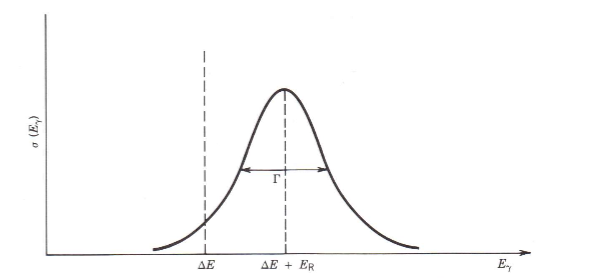
\includegraphics[scale=1.0]{images/resonance_recoil}
    \caption{Krane figure 10.23.~\cite{krane}.\label{fig:resonance_recoil}}
  \end{figure}
\item This has an exactly opposite effect on the emission
  spectrum. The absorption spectrum was shifted \textit{up} because the
  incoming photon needed extra energy to recoil the nucleus. The
  emission spectrum is shifted \textit{down} because the recoil takes some of
  the energy of the emitting photon.~\cite[Lec. 25]{lecture}
\item\textbf{Doppler broadening:} thermal motion makes the nuclei move back
  and forth, so the incoming photons energy looks doppler shifted
  either higher or lower. Therefore, a photon with energy just off the
  resonance may actually be absorbed because the relative motion can
  shift its energy to the resonance value. A wider energy range can
  now be absorbed by the resonance, so the peak gets wider or
  \textit{broadens}.~\cite[pp. 363]{krane}
\item Doppler broadening can can cause overlap between
  the emission and absorption peaks. ~\cite[Lec. 25]{lecture}
\item\textbf{Mossbauer Effect:} If a nuclei is in a crystal lattice,
  its recoil will be inhibited by the fact that \textit{its stuck in a
  lattice.} You're not just causing one nuclei to move, but
  all the ones around it, this makes the recoil energy very low, and
  therefore minimizes the shift in resonance energy by recoil. This
  allows you to nail down the \textit{actual} resonance
  energy.~\cite[Lec 25]{lecture}
\end{itemize}
\subsubsection{Giant Dipole Resonance}
High energy photons can ``ionize'' the entire nucleus by
  creating dipole motion between all the protons and all the
  neutrons. This means that all the protons moving together and all
  the neutrons are moving together, and these two groups are in a
  resonance with each other. This only occurs when the incoming photon energy is very
  high, $>$12 MeV.~\cite[Lec 25]{lecture}

\subsection{Coulomb Scattering}

\subsubsection{Elastic (Rutherford)}
\begin{itemize}
\item A particle approaches the nucleus at a distance $b$ (the impact
  parameter) and scatters off the coulomb potential. The particle
  follows a hyperbolic path.~\cite[pp. 396]{krane}
  \begin{figure}[hbtp]
    \centering
    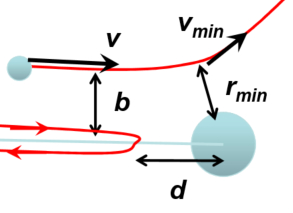
\includegraphics{images/rutherford}
    \caption{Geometry for elastic coulomb scatter.~\cite[Lec
      24]{lecture}}
    \label{fig:rutherford}
  \end{figure}

\item Based on the geometry in Figure~\ref{fig:rutherford}:

Incoming particle (at long distances):
\begin{equation*}
  \begin{split}
    V &= 0 \text{ (far away, the incoming particle has negligible
      potential energy)}\\
    T &= \frac{1}{2}mv^2 \\
    \ell &= mvb
  \end{split}
\end{equation*}
Target particle:
\begin{equation*}
  \begin{split}
    V &= \frac{Z_1Z_2e^2}{4\pi\epsilon_0}\frac{1}{d} \\
    T &= 0 \\
    \ell &= 0 \\
  \end{split}
\end{equation*}
Incoming particle (at the minimum distance $r_{min}$):
\begin{equation*}
  \begin{split}
    V &= \frac{Z_1Z_2e^2}{4\pi\epsilon_0}\frac{1}{r_{min}} \\
    T &= \frac{1}{2}mv_{min}^2 \\
    \ell &= mv_{min}r_{min}
  \end{split}
\end{equation*}
No energy or angular momentum is transferred to the target nucleus (hence elastic
scattering).~\cite[Lec 24]{lecture}
\end{itemize}

\subsubsection{Inelastic (Coulex)}
\begin{itemize}
\item \textbf{Coulomb Excitation:} inelastic Coulomb
  scattering. An incoming particle scatters off the potential of a
  target and leaves some energy behind. This ``Coulex'' reaction can
  excite nuclei up rotational bands.~\cite[Lec. 24]{lecture}
\item Reaction $Q$-value is to create the final products at rest.
  \begin{itemize}
  \item Center of Mass Frame: products are at rest, $Q = Q$.
  \item Lab Frame: products are \textit{not} at rest. Threshold energy
    for reaction is:
    \begin{equation*}
      E_{\text{threshold}}=Q\left(\frac{m_a+m_x}{m_x}\right)
    \end{equation*}
    for a(X,Y)b.
  \end{itemize}
\end{itemize}

\subsection{Direct Reactions}

\begin{itemize}
\item Occur on time frames of $10^{-21}-10^{-22}$s.~\cite[Lec
  25]{lecture}
\item These are collisions off the nucleons on the surface. They occur
  fast enough and with high enough energy that the incoming particle actually ``sees'' the
  individual protons and neutrons instead of the nucleus as a
  whole. This happens because the wavelength of the incoming particle
  is inversely proportional to momentum, and therefore energy:
  \begin{equation*}
    \lambda = \frac{h}{p}
  \end{equation*}
  So higher energy particles can interact with individual
  nucleons.~\cite[Lec 25]{lecture}
\item Different incoming angles affect the cross sections for
  reactions. This is because the incoming particle is a wave, and the
  nucleus is a big wave made up of little waves, so you can have
  constructive and destructive interference as the two interact. They
  can add up to make a reaction or less likely based on
  angle.~\cite[Lec 25]{lecture}
\end{itemize}

\subsubsection{Kinematics}
For an incoming particle $a$, outgoing particle $b$ and product,
  as shown in Figure~\ref{fig:direct_kinematics}
  \begin{figure}[hbtp]
    \centering
    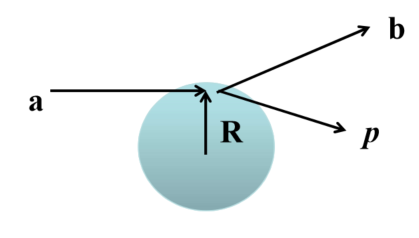
\includegraphics{images/direct_kinematics.png}
    \caption{Direction reaction kinematics diagram.\label{fig:direct_kinematics}}
  \end{figure}
The momentum is conserved:
\begin{equation*}
  \vec{p}_{product}=\vec{p}_a-\vec{p}_b
\end{equation*}
Based on the radius $R$ that the incoming particle comes in, there is
some amount of angular momentum $l$ transferred to the product
(spinning up the nucleus):
\begin{equation*}
  l=Rp
\end{equation*}
Using conservation of energy, you can also relate the final product
momentum ($p$) to the incoming and outgoing particles:
\begin{equation*}
  p^2=p^2_a+p^2_b-2p_a2p_b\text{cos}\theta
\end{equation*}
If you solve for $l$ you can figure out what $J^{\pi}$ the product
will be left in. In summary:
\begin{enumerate}
\item Figure out the momentum of the product using the momenta of the
  products and the angle of collision (that $p^2$ formula).
\item Solve for the angular momentum transfer $l$ using $R$ ($l=Rp$).
\item Add $l\pm\frac{1}{2}$ to the original $J^\pi$ of the target to
  get the final spin.
\item Parity change will go $\Delta\pi = (-1)^l$ where that $l$ is the
  angular momentum transfer from step 2.
\end{enumerate}
\cite[Lec 25]{lecture}

\subsection{Compound Reactions}
\begin{itemize}
\item Reactions with a definite intermediate state:
  \begin{equation*}
    a + X \to C^* \to Y + b
  \end{equation*}
Where $C^*$ represents the compound nucleus.~\cite[pp. 416]{krane}
\item Works best for particles with low incident energy (10-20 MeV),
  to reduce the chance the particle can escape with its energy and
  identity.~\cite[pp. 416]{krane}
\item Occur on time frames of $10^{-16}-10^{-18}$ seconds. The
  time-scale for decay is large compared to the time-scale for
  formation. This means that nuclei don't ``remember'' how they were
  formed; the formation process has no affect on what eventually
  happens to the nuclei (decay, etc). Only total energy and angular
  momentum information is retained.~\cite[Lec 26]{lecture}

\end{itemize}
\section{Neutron Physics}
\begin{itemize}
\item Free neutrons are unstable, they will $\beta$-decay into protons
  with a half-life of 10.6 minutes.~\cite[pp. 444]{krane}
\item Neutron energies are listed in
  Table~\ref{tab:neutron_e}.
\begin{table}[hbtp]
\centering
\begin{tabular}{ll}
           & Energy             \\
Thermal    & $\approx$ 0.025 eV \\
Epithermal & $\approx$ 1 keV    \\
Fast       & 100 keV - 10 MeV  
\end{tabular}
\caption{Neutron Energies~\cite[pp.445]{krane}}
\label{tab:neutron_e}
\end{table}

\subsection{Attenuation}

\begin{itemize}
\item As neutrons move through a material, they are absorbed and
  scattered, which will reduce the overall intensity of the beam. We
  consider scattered neutrons to be gone because they generally
  scatter away from the beam, so we don't see them anymore. Also, we
  usually define intensity with a given energy, so scattering lowers
  their energy and they leave our intensity.
\item The loss of intensity ($I$) of neutrons of a \textit{given
    energy} in a distance $dx$ of material:
  \begin{equation*}
    dI = -I\sigma_t n dx
  \end{equation*}
Where $\sigma_t$ is the total cross section of the material
(absorption plus scattering) and $n$ is the number of atoms per unit
volume of the material. To make this useful, solve:
\begin{equation*}
  I = I_0e^{-\sigma_tnx}
\end{equation*}
Where $x$ is the distance the neutrons are traveling through the
material. Remember, this isn't a decrease in the total number of
neutrons, just the ones in our beam with the amount of energy we shot
them into the material with. The scattering will make lower-energy
neutrons, so they aren't actually gone for reals.~\cite[pp. 448]{krane}
\end{itemize}

\subsection{Collisions}

\item The main process by which neutrons slow down (lose energy, also
  called the process of moderation) is collisions.
\item In an elastic collision with a nucleus of atomic mass $A$, a
  neutron with incoming energy $E$ will have final energy:
  \begin{equation*}
    \frac{E'}{E} = \frac{A^2 + 1 + 2A\text{cos}\theta}{{(A+1)}^2}
  \end{equation*}
\cite[pp.448]{krane}
\item The maximum energy loss is from a head-on collision ($\theta =
  180^\circ$), where the above equation reduces to:
  \begin{equation*}
    \left(\frac{E'}{E}\right)_{min} = {\left(\frac{A-1}{A+1}\right)}^2
  \end{equation*}
This is the ``min'' value because it's the minimum final energy ($E'$)
that the neutron can have after the collision. As $A$ gets larger, the
energy transferred goes down, the neutron just kind of grazes off. The
equation is maximized for $A=1$ (hydrogen) which is why water is so
good at moderating.~\cite[pp. 448]{krane}
\item We usually use the average energy lost after each collision
  (actually, the log of that amount), represented by squiggle
  ($\xi$) (This is actually the greek letter \textit{xi} but no one
  knows how to pronounce that. If you do, shut up it's squiggle now).
  \begin{equation*}
    \xi = {\left[\text{log }\frac{E}{E'}\right]}_{av}
  \end{equation*}
This can be related to the final energy after the neutron after $n$
collisions:
\begin{equation*}
  \text{log }E_n' = \text{log }E - n\xi
\end{equation*}
This is good for problems where you want to figure out how many
collisions are required to thermalize a neutron. There is a complex
equation for the value of $\xi$ assuming isotropic scattering:
\begin{equation*}
  \xi = 1 + \frac{{(A-1)}^2}{2A}\text{ log }\frac{A-1}{A+1}
\end{equation*}
For hydrogen ($A=1$), $\xi = 1$.~\cite[pp.449-450]{krane}
\end{itemize}

\subsection{Capture}
\begin{itemize}
\item Most of the time, neutron capture on most massive nuclei
  form compound nuclei.~\cite[Lec 26]{lecture}
\item Neutron capture immediately makes a nucleus with energy:
  \begin{equation*}
    E = S_n + E_n
  \end{equation*}
  Where $S_n$ is the neutron separation energy and $E_n$ is the energy
  of the incoming neutron.~\cite[Lec 27]{lecture}
\item Neutron capture rates are higher with higher $Q$ values. The $Q$
  value in this case is just equal to the neutron separation energy,
  $S_n$, so the higher $S_n$, the higher the chance of capturing a
  neutron. This is why capture rates near the ``valley of stability''
  are high, because $S_n$ is large.~\cite[Lec 27]{lecture}
\item Why does this happen? Nuclei like to go to states with lots of
  available transitions. The larger the $Q$-value, the more options
  the nuclei has for the decay that follows. Therefore, the higher the
  $Q$ value ($S_n$), the higher the chance of neutron
  capture.~\cite[Lec 27]{lecture}
\item You can figure out the energy and spin parity of the nuclei
  immediately following neutron capture. The final spin of the nuclei is:
  \begin{equation*}
    I' = I + \ell + s
  \end{equation*}
  and the parity change:
  \begin{equation*}
    \Delta\pi = (-1)^{\ell}
  \end{equation*}
If the neutron is thermal, the captured neutron will probably have no
angular momentum (``s-wave capture''). So $I' = I \pm \frac{1}{2}$;
unless $I=0$, in which it is always $I' = \frac{1}{2}$. Parity doesn't
change because $\ell = 0$.~\cite[pp.463]{krane}
\item After capture, the excited capture state will $\gamma$-decay down into all
  the accessible excited states of the compound nucleus. Many of them are
  accessible because $S_n$ is usually pretty high. Accessible means
  any states that the excited state can go to via \textit{E}1
  radiation, described below.~\cite[pp. 463]{krane}
\item After capturing a neutron, the primary transition that follows
  is dominated by Electric Dipole, \textit{E}1
  ($\Delta{}I=0 \text{ or } 1 \text{ and } \Delta\pi=-1$). The
  transition will populate all of these possible states. Magnetic
  dipole radiation and higher multipole radiation are usually present,
  but are usually far less intense than \textit{E}1. ~\cite[Lec
  27]{lecture}

  \vspace{10pt}
  Example: If neutron capture results in a compound nucleus in an
  energy state (at $S_n$) with $J^\pi = 2^+$, the following primary
  transition will populate states: $1^-, 2^-, 3^-$.
\item In summary:
  \begin{itemize}
  \item A neutron with energy $E_n$ is captured and makes a compound
    nucleus with energy $E=E_n + S_n$.
  \item The compound nucleus has a spin parity related to it's old
    spin-party ($I$) and the spin and angular momentum of the neutron.
  \item This excited compound nucleus will $\gamma$-decay via
    \textit{E}1 (electric dipole) radiation down to many other
    states. (Primary $\gamma$-rays)
  \item Unless it went down to the ground state, more decays will
    occur. (Secondary $\gamma$-rays)
  \end{itemize}
\end{itemize}
\section{Fission}

\section{Fusion}




\bibliographystyle{unsrt}
\bibliography{../NE101}
\end{document}
